\chapter{Introducción}
Según la Directiva General de la Comisión Europea para el Transporte y la Movilidad \cite{2}, en 2014, algo más de 25.700 accidentes de tráfico fueron informados en la Unión Europea. Aunque el número de accidentes se reduce sustancialmente, el informe sobre Transporte \cite{3} ha anunciado un objetivo estratégico para la seguridad en las carreteras europeas para el período de 2011 a 2020: reducir el número de muertes en carretera a la mitad. Si las estadísticas son analizadas, en el período de 2010 a 2012, el número de ciclistas muertos en siniestros ha aumentado un 6\%; siendo el único agente de la carretera cuyos resultados vayan a peor. Esto se explica, al menos parcialmente, por un aumento de la presencia ciclista en la carretera. Se podría decir que el ciclismo es un
medio de transporte donde los \gls{vru} tienen un mayor contacto con el tráfico de mayor afluencia y velocidad. Cuando están involucrados en un accidente, son los que sufren las consecuencias más graves derivadas de una colisión con otro agente de la carretera; ya que están completamente expuestos a otros vehículos.

Basados en estos estudios, los accidentes en la que están involucrados \gls{vru}s ocurren frecuentemente en vías diseñadas para viandantes y ciclistas; por ejemplo en pasos de peatones y caminos para ciclistas cercanos a infraestructuras comunes de tráfico, las carreteras. Por lo tanto, la pregunta es: ¿Cómo se pueden reducir los accidentes de \gls{vru}s, y cómo minimizar la gravedad de un siniestro y sus consecuencias? Se pueden tomar varias soluciones: mejorar el diseño y trazado de las vías de comunicación, mejorar la iluminación, instalar más infraestructuras de protección, promocionar equipamiento de seguridad y enseñar cómo utilizarlo...

Sin embargo, hay otras soluciones viables aparte del re-diseño de las infraestructuras existentes, o soluciones pasivas como el uso del casco de seguridad. Una opción que está ganando fuerza en los países desarrollados es el desarrollo de soluciones para la movilidad
en el entorno de ciudades inteligentes. Aunque el término de ciudad inteligente pueda parecer confuso, se podría decir que se considera \emph{inteligente} cuando se ha aplicado tecnologías de la información y comunicación para mejorar la calidad de vida en áreas como la seguridad, gasto energético, reducción de costes, y gobierno y transporte, permitiendo una participación efectiva y activa por parte de los ciudadanos.

En el dominio de las ciudades inteligentes, las soluciones para transporte diseñadas tratan de hacer un uso más seguro, sostenible y eficiente de la carretera a través de un mejor entendimiento del estado de tráfico, la posición de los los vehículos y usuarios, y el
registro de eventos que suceden durante el transporte. Estas soluciones combinan la capacidad y beneficios de los sensores, dispositivos, infraestructura física y arquitecturas de comunicación combinada con sistemas de información en la nube, y la capacidad de analizar grandes volúmenes de datos.

En este contexto, los \gls{its} emergen como una respuesta tecnológica para una mejor motorización y caracterización del tráfico. Estos sistemas permiten al mismo tiempo mejorar el uso y eficiencia de la carretera, así como la seguridad de los usuarios, particularmente aquellos definidos como vulnerables; ciclistas, peatones o motoristas. Los ITS actuales requieren el uso de cámaras de tráfico, paneles informativos, o sensores de inducción que obtengan datos para ser posteriormente mandados y procesados en la central de gestión de tráfico. A diferencia de estas soluciones que requieren el uso de sensores, actualmente surgen sistemas conocidos como \gls{fcd}, que se encargan de reunir información de los \gls{gps} obtenidos de terminales móviles y el uso de páginas web colaborativas como Waze, que permite a los conductores obtener y proveer información sobre la carretera sin necesidad de ningún sensor en la carretera. Este tipo de soluciones basadas en \gls{fcd} tienen a favor la motorización del estado de los usuarios de manera ubicua, pero su fiabilidad depende del número de vehículos y usuarios informando sobre los eventos y aportando datos.

En el dominio de los \gls{its}, los \gls{cits} son sistemas que permiten la conexión directa entre vehículos (comunicaciones \gls{v2v}) o entre vehículos e infraestructuras (comunicaciones \gls{v2i}) para intercambiar de información con el objetivo de mejorar la seguridad vial y la gestión del tráfico. Estos enlaces son posibles gracias a las \gls{obu}, dispositivos \gls{cits} dedicados que habilitan interfaces de comunicación, y dispositivos localizados en infraestructuras llamados \gls{rsu}.

La importancia de las tecnologías \gls{cits} para la administración pública y la comisión europea se ve reflejada en la directiva 2010/40/EU, donde la \gls{eu} reconoce la capacidad de los \gls{cits} para mejorar la gestión actual del tráfico y conducir los procesos de implementación y desarrollo de estos sistemas en las infraestructuras de las carreteras europeas. Tras docenas de proyectos de I+D como \gls{cvis}, \gls{team}, el desarrollo masivo de sistemas \gls{cits} está más cerca. Un ejemplo es el \gls{mou} firmado por la industria automovilística y las organizaciones de infraestructuras con el objetivo de desplegar soluciones basadas en \gls{cits} en 2015. Las administraciones públicas también están trabajando en la misma dirección, resaltando el acuerdo alcanzado en Alemania, Austria y Holanda para desplegar un ''pasillo'' entre estos tres países equipados con tecnologías \gls{cits}. Merece la pena recalcar el anuncio publicado en Febrero del 2014 por la \gls{nhtsa}, perteneciente al \gls{usdot}, de su intención de tomar los pasos necesarios para el despliegue de sistemas cooperativos \gls{v2v} en los años venideros, concretamente desde 2017, para vehículos comerciales.

En un escenario \gls{cits}, hay generalmente cuatro agentes a considerar: dos entidades móviles (\gls{obu}s y peatones), y dos entidades estacionarias (la \gls{rsu} y el sistema central). Estas entidades son capaces de ejecutar cuatro tipos diferentes de aplicaciones: seguridad activa en la carretera, tráfico eficaz cooperativo, servicios locales cooperativos, y servicios globales en Internet. Sobre cada tipo, hay diferentes definiciones de casos de uso y aplicaciones, donde cada agente puede ser considerado un sensor que genera información. Dependiendo de la aplicación y las restricciones de  tiempo, el intercambio de información entre las entidades se puede clasificar como:

\begin{description}
	\item Mensajes de alerta: se definen como notificaciones descentralizadas y pueden ser enviados desde cada vehículo o \gls{rsu}.

	\item Mensajes periódicos o ''beacons'': son usados por los \gls{obu} para notificar su posición, velocidad e identidad a las RSU que forman parte del \gls{fcd}. Además, estos mensajes también son usados para conocer la situación	actual del tráfico. Por ello, el Acceso Inalámbrico en Entornos Vehiculares (\gls{wave})	define los Mensajes de Aviso Cooperativo (\gls{cam}s), que son transmitidos periódicamente	a todos los vehículos en área de alcance.

	\item Mensajes sobre infotainment: notificaciones no relacionadas con la seguridad, sino que son usados para aportar mayor información y confort al conductor; datos turísticos, acceso a Internet, asistencia en navegación, etc.
\end{description}

En el campo de los servicios \gls{cits}, una gran variedad de aplicaciones y casos de uso se centran en incrementar la seguridad del usuario. Teniendo en cuenta requisitos estratégicos, económicos y de organización, características del sistema así como requisitos legales y de estandarización, el Comité del Instituto Técnico Europeo de Estándares en la Telecomunicación ha definido un conjunto básico de aplicaciones para usar como referencia en ITS para desarrolladores \cite{6}. Entre ellos, los Avisos a Usuarios Vulnerables en Carretera tratan de proveer notificaciones a los vehículos sobre la presencia de usuarios vulnerables, por ejemplo ciclistas, y en caso de existir situaciones de peligro también se avisa a los VRU sobre la presencia de un vehículo cercano.

Siguiendo los requisitos presentados por el ETSI, este proyecto presenta un sistema que emplea a los vehículos y ciclistas como sensores móviles que aportan información sobre su posición, velocidad y rumbo con el objetivo de detectar la proximidad entre estas dos entidades y avisarles en el caso de detectar peligro. Esta solución tiene un sistema centralizado que despliega comunicación inalámbrica vehicular, conectividad móvil y computación en la nube, y gestiona la información obtenida por los usuarios (vehículos y ciclistas). El sistema ha sido desplegado y verificado en un dominio real, y se han realizado pruebas de rendimiento en diferentes escenarios para comprobar el correcto funcionamiento de las comunicaciones en los peores escenarios. Actualmente, existe un proyecto llamado \gls{icsi}, con similares aplicaciones que se encuentra bajo desarrollo usando una solución descentralizada con la finalidad de mejorar el rendimiento y la seguridad.

\section{Estado del arte}\label{section:antecedentes}
Las aplicaciones para la detección de \gls{vru} no son un nuevo tema. Durante muchos años, se han desarrollado sistemas que han empleado diferentes técnicas para detectar principalmente peatones. El reconocimiento de imágenes es probablemente el campo científico en el que se han realizado mayores esfuerzos para minimizar el impacto de posibles accidentes entre peatones y vehículos. En [6]m Takahashi \emph{et al.} implementaron un entorno de clasificación de usuarios de carretera urbanos empleando descripciones de características locales y modelos ocultos de Markov (HMM) para detectar peatones, ciclistas y motociclistas. En la aproximación definida por Fardi \emph{et al.} [7], se ha definido un sistema multisensor basado en sensores al lado de cámaras infrarrojas y \gls{wpan}, proveyendo un seguimiento de \gls{vru}s en un rango de 60 metros.

Otras aplicaciones están basadas en sistemas de radares. Por ejemplo, Heuel \emph{et al.} [8] fueron capaces de medir el rango del objetivo y la velocidad radial gracias a un radar de 24 GHz desplegado en la parte superior del vehículo. Por otra parte, Schaffer \emph{et al.} [9] proponen un sistema más complejo que emplea un esquema de radar secundario para detectar y localizar \gls{vru}s, infraestructuras y otros vehículos equipados con emisores de radio con la intención de mejorar la seguridad vial, incluso sin tener puntos muertos.

Aplicaciones como [10-12] han sido configuradas en base al intercambio de datos entre vehículos y \gls{vru} empleando dispositivos nómadas, pero usando, en cualquier caso, plataformas con comunicación de corto alcance y sin combinar enlaces de corto y largo alcance como en el presente proyecto. En otros casos, estas aproximaciones no han sido consideradas aplicaciones cooperativas ya que no soportan la comunicación entre diferentes usuarios de la carretera.

Sin embargo, las soluciones basadas en sensores tienen problemas para operar de noche o en condiciones de baja visibilidad, con mal tiempo, o si los \gls{vru} no están lo suficientemente cerca o en un punto muerto del sensor. Además, muchos de estos sitemas están centrados en solo detectar al \gls{vru} desde la perspectiva del vehículo; por lo que tan solo el éste es avisado sobre la presencia del
\gls{vru}, y por lo tanto es el único que puede realizar maniobras preventivas. Además, estos sistemas requieren de un despliegue de no solo sistemas complejos de sensores sino de equipos de procesamiento capaces de procesar una alta cantidad de datos a tiempo real. Este proyecto ha sido diseñado para emplear las características y las capacidades de procesamiento de dispositivos habituales, como los smartphones y sencillos servidores, para minimizar los requisitos de complejos y caros dispositivos. Esta aproximación también ha sido elegida para conseguir una rápida penetración en el mercado de este tipo de aplicaciones sin la implicación de fabricantes de automóviles; lo cual es necesario para desplegar cualquier hardware integrado a bordo. Es verdad que se han empleado unidades de comunicación \gls{ieee} 802.11p, pero de hecho se espera que esta tecnología sea la que provea de comunicaciones inalámbricas a los vehículos combinando comunicaciones de largo alcance como \gls{lte}[13].

\section{Primera aproximación}
Como se ha mencionado en la introducción, el objetivo principal de este proyecto es evitar accidentes que involucre \gls{vru}s en un escenario urbano. Aunque la solución propuesta es completamente funcional, tan solo ha sido probada a pequeña escala. Para intentar obtener el comportamiento que esta solución tendría en escenarios más complejos, se ha decidido probar la aplicación en un escenario simulado con más vehículos (4), más ciclistas (8), y modelando los parámetros de comunicaciones; los cuales son críticos para la fiabilidad de la aplicación.
\begin{figure}[t]
	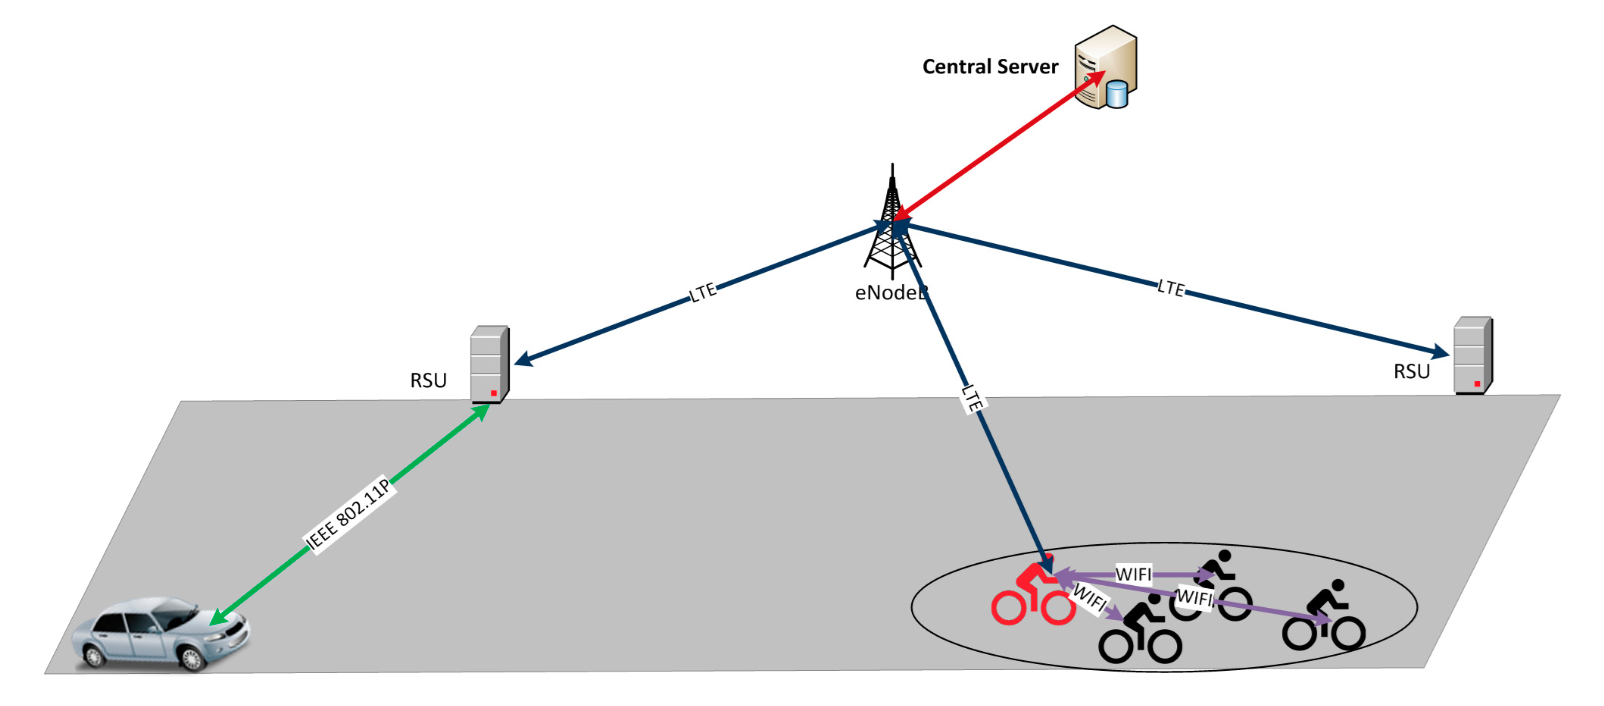
\includegraphics[scale=0.6]{simulacion-vehiculos}
	\caption{Descripción de la arquitectura simulada}
	\label{fig:simulacion-vehiculos}
\end{figure}
En la figura \ref{fig:simulacion-vehiculos} se muestra la arquitectura diseñada para validar el rendimiento de la solución en un sistema \gls{fcd} por medio de una simulación. Esta arquitectura permite el intercambio de información entre sensores móviles (obtenidos de vehículos y ciclistas) gracias a un servidor central que tiene una visión global del escenario en carretera.

Esta variedad de tecnologías en la arquitectura permite la ejecución de tres fases principales:
\begin{enumerate}
	\item Obtención de datos: esta fase consta de todo lo relacionado con enviar información al servidor central. Por lo tanto, por una parte, como todo vehículo actúa de sensor mandando \gls{cam}s, cada \gls{rsu} es capaz de conocer la información sobre la posición de todos los vehículos que se encuentran en su área de cobertura y retransmite esta información al servidor central. Por otra parte, las bicicletas también están enviando mensajes periódicos con la información sobre su posición dentro de una red Wi-Fi; por consiguiente, el líder de los ciclistas es capaz de reunir toda esta información sobre el grupo y enviarla al servidor central a través de tecnología \gls{lte}.
	
	\item Gestión de información centralizada: la recepción de información actualizada sobre la situación en carretera por el servidor central permite comprobar qué vehículos pueden encontrarse con un grupo de ciclistas e informar a las bicicletas sobre la posición de los vehículos.
	
	\item Dispersión de mensajes de alerta: esta fase está encargada de enviar información de los vehículos a los ciclistas, y la información de los ciclistas a los vehículos. Por consiguiente, el servidor central envía la información de los ciclistas al \gls{rsu} a través de \gls{lte}, y las \gls{rsu} dispersan esta información a través de de IEEE 802.11p con el objetivo de ser recibidos por los vehículos interesados en su área de cobertura. Al mismo tiempo, el servidor envía información sobre los vehículos que se aproximan al líder de ciclistas por medio de \gls{lte} y el líder de ciclistas dispersa esta información al resto de ciclistas a través de Wi-FI.
\end{enumerate}
\subsection{Configuración de la simulación}
El objetivo principal de la simulación es mostrar la viabilidad y el rendimiento de la arquitectura anteriormente propuesta. Por lo tanto, esta arquitectura es evaluada empleando un simulador en red de eventos discretos NS-3 [14], el cual es open source y validado por la comunidad de investigación. Además, NS-3.21 provee de modelos para la asistencia de redes vehiculares heterogéneas, incluyendo modelos de comunicaciones de corto alcance como Wi-Fi y IEEE 802.11p y redes móviles como \gls{lte}. Para generar las rutas que realizarán los vehículos y bicicletas durante la simulación NS-3, se emplea el simulador de tráfico\gls{sumo} [15]. El escenario simulado es un área suburbana de Bilbao donde hay normalmente hay múltiples grupos de ciclistas y el flujo de vehículos es irregular. Los vehículos y bicicletas se mueven durante 600 segundos en una carretera de 5 km. La tabla     detalla los detalles de la simulación empleados durante la evaluación.

\begin{table}[H]
	\centering
	\caption{Tipo de mensajes en grupo}\label{tab:parametros_simulacion}
	\begin{tabular}{lll}
		\toprule
		\textbf{Tipo} & \emph{Parámetro} & Valor \\
		\midrule
		Vehículos	&	Frecuencia \gls{cam}	&	1 Hz \\
		\gls{rsu}	&	Frecuencia de actualización TMC	&	Mensaje \gls{cam} recibido por el vehículo \\
		Bicicleta	&	Frecuencia de actualización del líder	&	1 Hz \\
		Bicicleta líder & Frecuencia de actualización TMC	& 1 Hz \\
		\midrule
		\multirow{5}{*}{Escenario}	&	Tipo	& Suburbano \\
													&	Número de vehículos	&	4	\\
													&	Número de ciclistas &	8	\\
													&	Velocidad del vehículo	&	10-70 km/h \\
													&	Velocidad del ciclista	&	25-30 km/h \\
		\midrule
		\multirow{5}{*}{Red IEEE 802.11p} &	Bit rate	&	3 Mbps \\
													&	Banda ancha	&	10 MHz \\
													&	Banda de frecuencia	&	5.9 GHz \\
													&	Potencia máxima de TX	&	21 dBm \\
													&	Modelo de propagación	&	Nakagami \\
		\midrule
		\multirow{5}{*}{Red IEEE 802.11b} &	Bit rate	&	1 Mbps \\
													&	Banda ancha	&	20 MHz \\
													&	Banda de frecuencia		&	2.4 GHz \\
													&	Potencia máxima de TX	&	16 dBm \\
													&	Modelo de propagación	&	Nakagami \\
		\bottomrule
	\end{tabular}
\end{table}

\subsection{Mediciones y resultados}
Las siguientes mediciones son considerados en este estudio:
\begin{itemize}
	\item Retraso en la recepción de los ciclistas (ms): el tiempo que ha pasado entre que el mensaje ha sido transmitido por el vehículo y la recepción del mensaje por el ciclista.
	
	\item Retraso en la recepción de los vehículos (ms): el tiempo que ha pasado entre que el mensaje ha sido transmitido por el líder ciclista y lo ha recibido el vehículo.
\end{itemize}

\begin{figure}[t]
	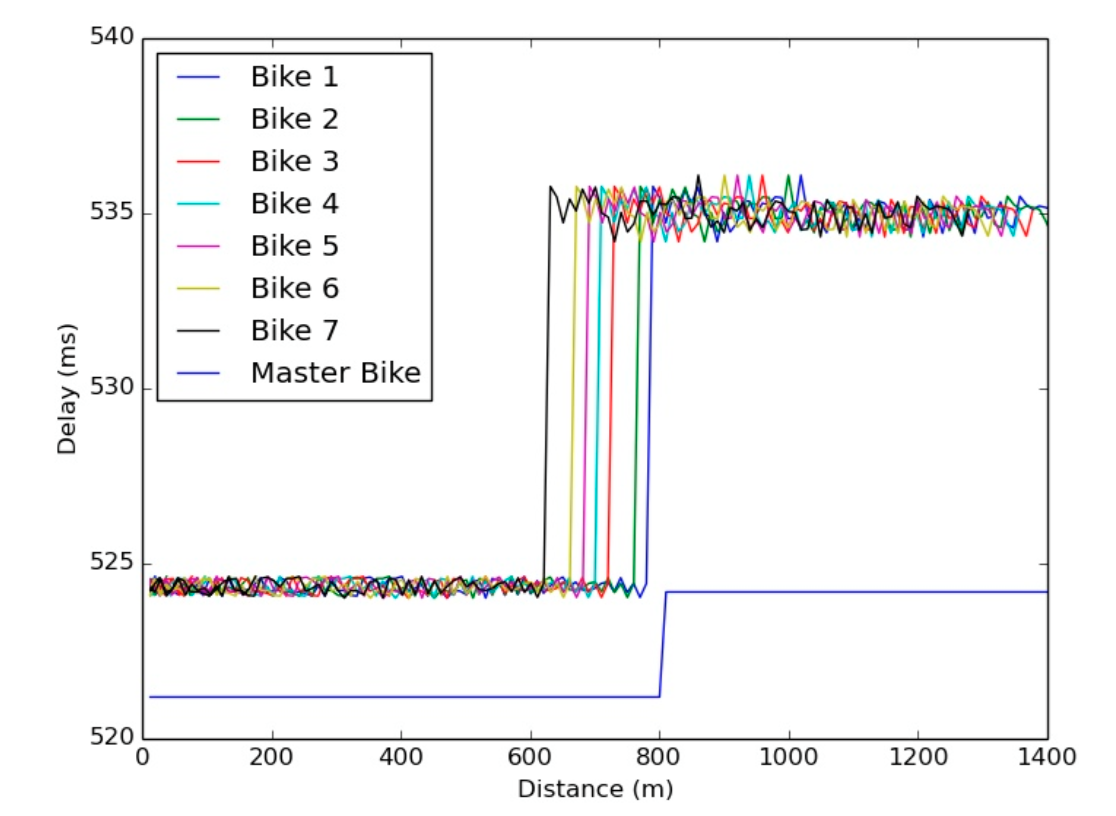
\includegraphics[scale=0.6]{delay-recepcion-ciclista}
	\caption{Retraso en recepción del ciclista}
	\label{fig:delay-recepcion-ciclista}
\end{figure}

\begin{figure}[t]
	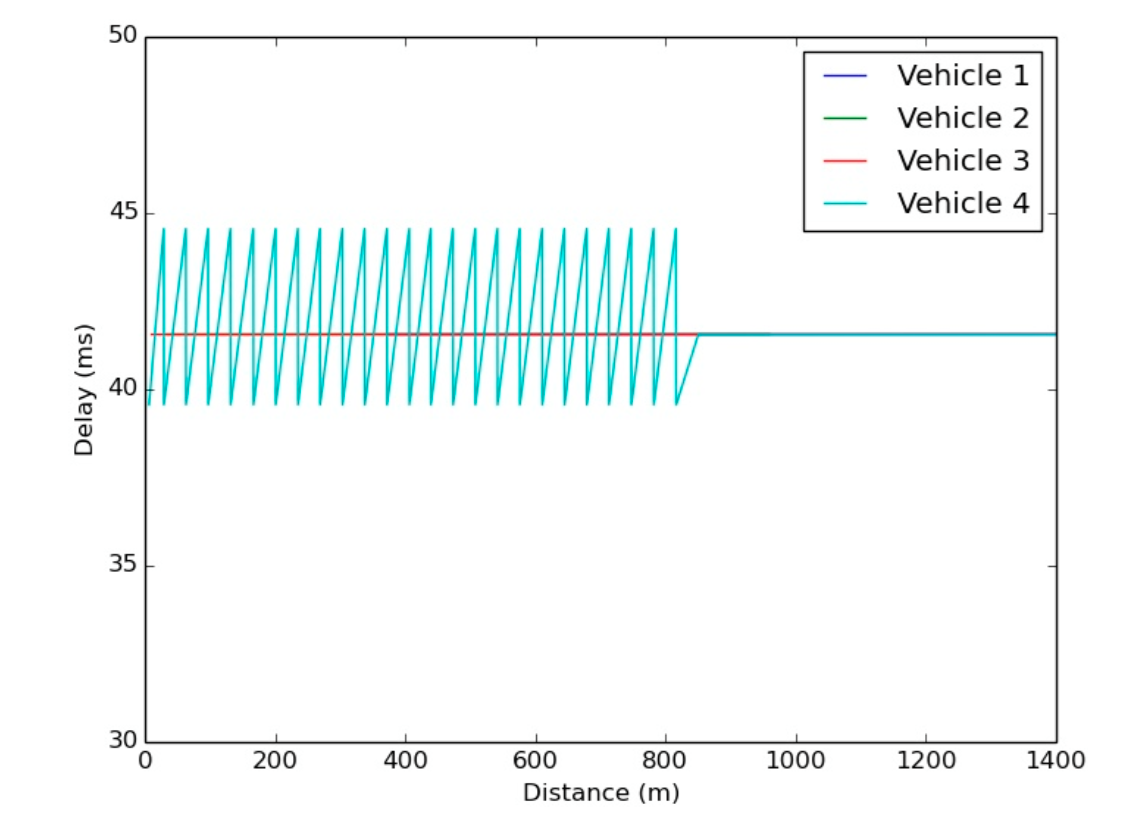
\includegraphics[scale=0.6]{delay-recepcion-vehiculo}
	\caption{Retraso en recepción del vehículo}
	\label{fig:delay-recepcion-vehiculo}
\end{figure}

La validación de los resultados de la simulación es necesaria para desplegar la aplicación en entornos reales. La fiabilidad depende del retraso del mensaje de alcanzar el destino. Por lo tanto, la figura \ref{fig:delay-recepcion-ciclista} muestra la media de retraso de un mensaje que sale de un vehículo a una bicicleta dependiendo de la distancia entre el vehículo y la bicicleta. Como se muestra en la figura \ref{fig:delay-recepcion-ciclista}, el tiempo que un mensaje necesita para alcanzar al líder de la bicicleta es menor que el resto de bicicletas porque el líder es el encargado de dispersar el mensaje del vehículo al resto de bicicletas a través de la red Wi-Fi. La figura \ref{fig:delay-recepcion-vehiculo} muestra el retraso de recepción del vehículo, que es casi constante para todas las distancias.

Comparando los resultados de las figuras \ref{fig:delay-recepcion-ciclista} y \ref{fig:delay-recepcion-vehiculo}, se puede observar que el retraso de recepción de la bicicleta está en un rango de entre 522 ms y 535 ms, pero la media de retraso de recepción de un vehículo es de 40 ms. Esta diferencia es debida a la ruta que cada mensaje tiene que seguir y la frecuencia de actualización del \gls{tmc} en el \gls{rsu} y líder de ciclistas.

El retraso de recepción en el ciclista está definido en la ecuación \ref{eq:delay_lider} para el líder de ciclistas y en la ecuación \ref{eq:delay_seguidores} para el resto de bicicletas en el grupo (seguidores):
\begin{equation}\label{eq:delay_lider}
D_{lider} = D_{v-RSU} + D_{RSU-TMC} + D_{TMC-BM}
\end{equation}

\begin{equation}\label{eq:delay_seguidores}
D_{seguidores} = D_{v-RSU} + D_{RSU-TMC} + D_{TMC-BM} + D_{BM-B}
\end{equation}
donde
\begin{itemize}
	\item $D_{v-RSU}$ es el tiempo desde que el mensaje ha sido generado en el vehículo hasta que el \gls{rsu} recibe dicho mensaje.
	
	\item $D_{RSU-TMC}$ es el tiempo que pasa desde que el \gls{rsu} recibe el mensaje desde el vehículo hasta que es recibido por el \gls{tmc}.
	
	\item $D_{TMC-BM}$ es el tiempo que pasa desde que el \gls{tmc} recibe el mensaje desde la \gls{rsu} hasta que es recibido por el líder.
	
	\item $D_{BM-B}$ es el tiempo que pasa desde que el líder recibe el mensaje del \gls{tmc} hasta que es recibido por los ciclistas que están en la red Wi-Fi.
\end{itemize}
El retraso de la recepción por el vehículo está definida por la ecuación \ref{eq:delay_vehiculo}:
\begin{equation}\label{eq:delay_vehiculo}
D_{vehículo} = D_{BM-TMC} + D_{TMC-RSU} + D_{RSU_V}
\end{equation}
donde
\begin{itemize}
	\item $D_{BM-TMC}$ es el tiempo que pasa desde que el mensaje es generado en el líder de ciclistas hasta que es recibido por el \gls{tmc}.

	\item $D_{TMC-RSU}$ es el tiempo que pasa desde que el mensaje es recibido por el \gls{tmc}, enviado por el líder de ciclistas, hasta que es recibido por el \gls{rsu}.
	
	\item $D_{RSU-V}$ es el tiempo que pasa desde que el \gls{rsu} recibe el mensaje procedente del \gls{tmc}, y es recibido por el vehículo.
\end{itemize}

La diferencia viene dada porque el \gls{tmc} solo envía mensajes de alerta las \gls{rsu}s y al líder de ciclistas cuando recibe un mensaje de un vehículo. Como el grupo de ciclistas está actualizando la información del \gls{tmc} a través del líder de ciclistas a una frecuencia de 1 Hz, como se muestra en la figura \ref{fig:simulacion-diagrama-secuencia}, hay un retraso desde que el \gls{rsu} recibe un mensaje desde el vehículo hasta que lo retransmite al \gls{tmc}. Sin embargo, este retraso no existe desde el líder de ciclistas hasta el \gls{tmc} ya que el líder de ciclistas está generando un nuevo mensaje con la información del grupo de ciclistas.

\begin{figure}[t]
	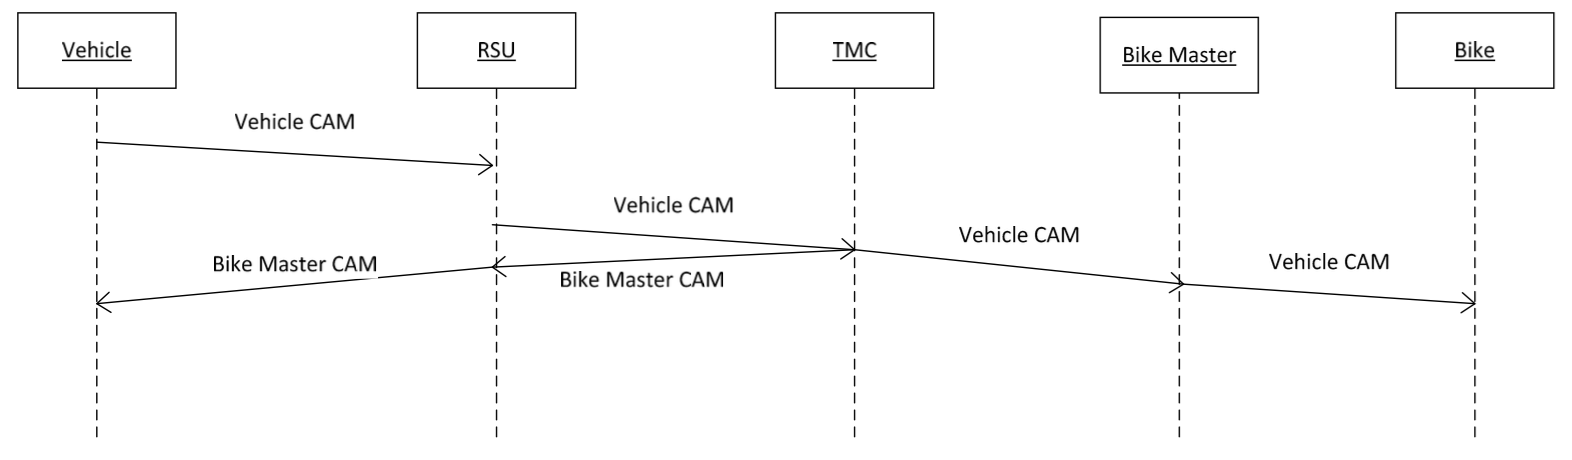
\includegraphics[scale=0.6]{simulacion-diagrama-secuencia}
	\caption{Diagrama de secuencia del sistema}
	\label{fig:simulacion-diagrama-secuencia}
\end{figure}